\Section{On-chain Atomic swaps}
Onchain atomic swaps is a method where two parties can exchange cryptocurrencies between different chains in an atomic way, in this case it means that none of the parties can cheat the other and no matter what state in the exchange-process the swap is either completed or reversed entirely, to the pre-exchange state. The onchain distinction comes from the fact that this type of atomic swap occurs entirely on the chains (There is no offchain transaction in the process).

There are several ways atomic swaps can be performed, scripts, signatures and time locks can take several different combinations in transactions and still retain atomicity. The method that will be described in this report will be a P2SH, pay to contract type. This swap is done with the help of time locked contracts constructed with scripts. 

\Subsection{The contracts}
A swap contract contains certain components. The initial component is the secret $x$ that is generated by the initial contract creator. The secret is not included in the initial contract however, this is what is included:
\begin{itemize}
	\item Byte string $h$ \quad - \quad Hash of secret $x$
	\item Integer $T$ \quad\quad - \quad Contract expiration time as timestamp
	\item Address $B$ \quad - \quad Redeemer address
	\item Address $A$ \quad - \quad Refund address
\end{itemize}

The contract uses branching provided by the operations \texttt{OP\_IF}, \texttt{OP\_ELSE} and \texttt{OP\_ENDIF}. The branch that is taken during execution is decided by whoever is trying to spend the output. One branch pays to the redeemer address, for it to be valid the secret has to be revealed. The other branch pays to the refund address, but it can only be valid if the current time is equal to or greater than the timestamp T.

\Subsubsection{Counter party contract}
The contract described above is the one constructed by and broadcast by whoever wants to initialize the exchange. A very similar contract has to be constructed and broadcast by the counter party, this contract however contains a few changes. The only variable that remains unchanged is $h$. $T$ has to be be a value between the current time and $T$ from the old contract, denoted $T/2$. Redeemer and refund addresses has to be changed so that the redeemer is whoever constructed the initial contract and the refund address is yourself.

\Subsection{The process}
Imagine Alice and Bob wants to swap cryptocurrencies. Alice has Bitcoin and wants Litecoin, Bob vice versa. Alice is the initiator in this case. The process would be the following:
\begin{enumerate}
	\item Alice generates a new secret and then constructs a contract from the variables needed as stated above.
	\item She broadcasts a p2sh transaction (to the Bitcoin blockchain) that pays to the constructed contract, called the contract transaction. Alice then sends the contract and the contract transaction txid to Bob.
	\item Bob fetches the transaction from the Bitcoin blockchain and validates all the variables, as well as the contract to contract hash etc\dots
	\item If all seems to be in order, Bob can construct his own contract using the same secret hash h as Alice did in her contract. This time however the timelock is set to $T/2$. He then broadcasts a transaction paying to the contract on the Litecoin network. Just as Alice did, Bob sends the contract and txid to Alice.
	\item Alice validates all the data the same way that Bob did in step 3. 
	\item If all seems to be in order. Alice could claim the Litecoins from Bobs contract transaction by making a transaction spending the output. The input that validates the output script must contain the secret x to be valid.
	\item Meanwhile Bob monitors the Litecoin chain for someone spending his contract transaction. If somebody does it means that they know the secret $x$. Any information in the blockchain can be extracted, Bob needs to know $x$ to spend Alice's contract transaction. If somebodies spends his contract transaction he can extract $x$ from that and spend the Bitcoin side transaction.
\end{enumerate}

\Subsubsection{Visualizer}
The next page contains a diagram visualizing the process described above. T is set to 48 hour after initialization in the example, thus T/2 would be 24 hours.

\Subsection{Atomicity}
Easiest way to show the atomicity of the swap is to show what happens if one party stops cooperating during any step in the process. The two trivial cases are before any step in the process, then no transaction has been made and the state did not change at all. If one becomes uncooperative at the end of the process the state change has already been completed and it doesn't matter what anyone does. The non-trivial cases is when someone becomes uncooperative mid process.\\

\InsertBoxR{0}{
	\footnotesize\setlength\fboxsep{10pt}\setlength\fboxrule{1pt}
	\fcolorbox{IndianRed3}{SlateGray1}{\begin{minipage}{2.1in}
			\subsection*{Can Alice wait to the last second before she claims the Litecoins?}
			Yes, but remember that Bob's contract expires before Alice's contract does: $T > T/2$, Even if Alice waits to the very last second, Bob will still have an equal amount of time to claim Alice's Bitcoins after that.
	\end{minipage}}
}[4]

The first case we will look at is if Bob stops responding after step 2. Meaning he never broadcasts his side of the contract. Then Alice simply never reveals $x$, Bob needs $x$ to claim the Bitcoins. Alice then just waits until timelock $T$ has passed and refunds the transaction. After the refund the state has been reset to the initial state.

The second case is if Alice becomes unresponsive after Bob has broadcast his side of the contract. Bob can't do anything until he knows $x$ or the timelock ($T/2$) of his transaction expires. If Alice does nothing Bob will never know $x$ and thus has to wait to refund his transaction. Presumably Alice does the same after timelock $T$ expires. The state has been reset to the initial one.

\newpage
\centerline{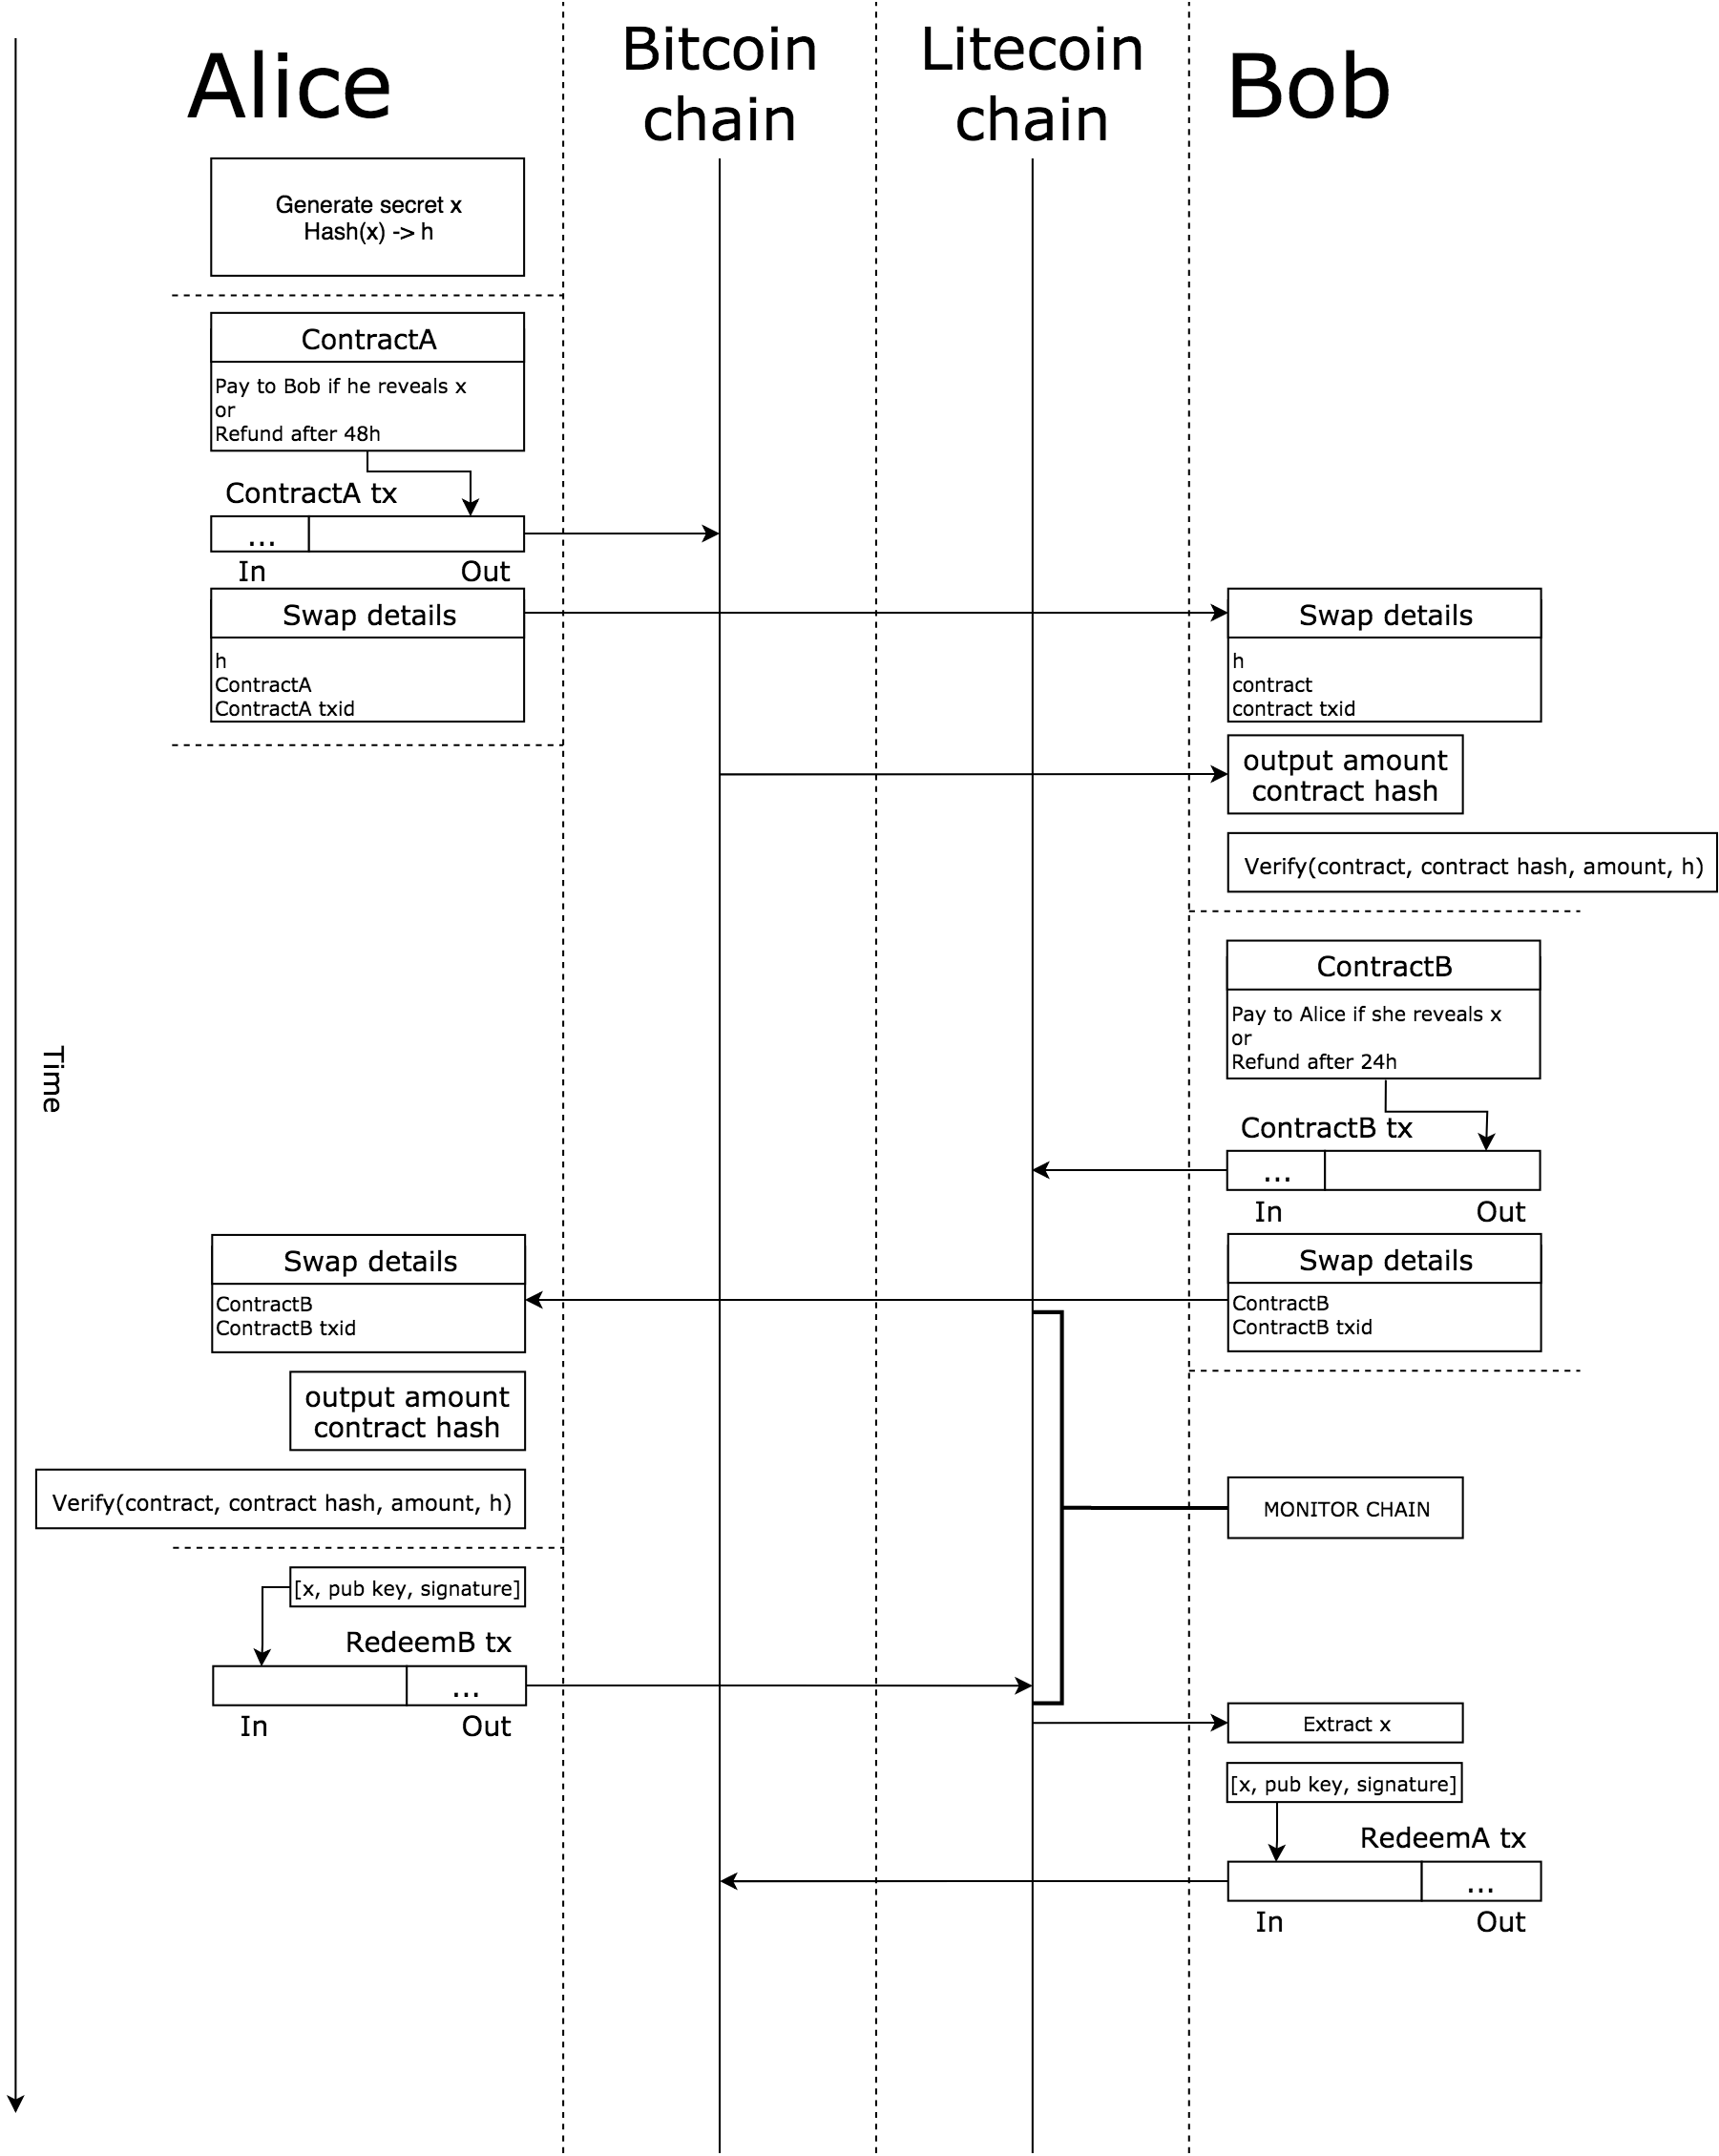
\includegraphics[width=1.35\textwidth]{background/images/atomic_swap_flow_large.png}}
\newpage

\Subsection{How the swap could fail}
The atomicity of the swap depends on each party acting rationally and not doing any mistakes that compromises the process. For example if Alice broadcasts her side of the contract and then reveals $x$ to Bob thorough some alternative communication channel then Bob could claim the Bitcoins without doing his part of the deal. 

Malformed contracts could also lead to money being stolen. This is why the validation steps are very important. For example Alice could maliciously set her contract to expire earlier than Bobs if Bob is not careful.

Actors in the scenario doing nothing also compromises the swap. If Alice waits until after $T/2$ expires before attempting to claim the Litecoins she is risking out on losing both the currencies. Bob could monitor the transaction pool, seeing what $x$ was, then sneak in his own refund transaction reclaiming his Litecoins (This is possible as the refund branch of the contract now is unlocked). Then also claiming the Bitcoins before $T$ expires.